\documentclass[12pt]{article}
\usepackage{latexblog}

% ============================================================
% Blog Metadata
% ============================================================
\blogtitle{浅析Java中的InvokeDynamic}
\blogdate{2019-12-24}
\blogtags{刨根问底, 探索分析, JVM}
\bloglang{zh}
\blogsummary{}

\begin{document}
\makeblogtitle

Java语言在被编译成class文件后，在class文件中，有专门的一个\href{https://docs.oracle.com/javase/specs/jvms/se7/html/jvms-4.html\#jvms-4.4}{``常量池''(Constant Pool)}区域来存储一些运行所需要的常量，包括一些写死的变量（比如定义一个字符串\texttt{String\ str\ =\ "Hello\ world"}以及一些符号，例如类和方法的的名称等）。在JVM(se7)规范中，有以下这些类型的常量：

\begin{Shaded}
\begin{Highlighting}[]
\ExtensionTok{CONSTANT\_Class}\NormalTok{                           CONSTANT\_Long            }
\ExtensionTok{CONSTANT\_Fieldref}\NormalTok{                        CONSTANT\_Double          }
\ExtensionTok{CONSTANT\_Methodref}\NormalTok{                       CONSTANT\_NameAndType     }
\ExtensionTok{CONSTANT\_InterfaceMethodref}\NormalTok{              CONSTANT\_Utf8            }
\ExtensionTok{CONSTANT\_String}\NormalTok{                          CONSTANT\_MethodHandle    }
\ExtensionTok{CONSTANT\_Integer}\NormalTok{                         CONSTANT\_MethodType      }
\ExtensionTok{CONSTANT\_Float}\NormalTok{                           CONSTANT\_InvokeDynamic       }
\end{Highlighting}
\end{Shaded}

大部分我们顾名思义，都可以知道是大概是干啥的，比如字符串啊，数字啊，方法名称之类的；但是可以注意到最后面一个是称之为\texttt{CONSTANT\_InvokeDynamic}的常量，这个就有点陌生了。那么，这是一个什么样的常量？什么情况下会出现这个呢？

\section{\texorpdfstring{\texttt{invokedynamic}指令}{invokedynamic指令}}\label{invokedynamicux6307ux4ee4}

在JVM规范中有说，\texttt{CONSTANT\_InvokeDynamic}常量是用来给\texttt{invokedynamic}指令指定一系列的参数的，那么有必要先了解一下\texttt{invokedynamic}这个指令了。这是Java 7引入的一个新指令，也是自Java 1.0以来第一次引入新的指令。

\subsection{\texorpdfstring{Java7之前的\texttt{invoke-}指令}{Java7之前的invoke-指令}}\label{java7ux4e4bux524dux7684invoke-ux6307ux4ee4}

实际上，在此之前，已经有一些列的\texttt{invoke}开头的指令了：

\begin{itemize}
\tightlist
\item
  \texttt{invokevirtual}：用来调用类的实例方法，也就是最普遍的方式
\item
  \texttt{invokestatic}：用来调用静态方法
\item
  \texttt{invokeinterface}：用来调用通过接口调用的方法
\item
  \texttt{invokespecial}：用来调用一些编译时就能够确定的，包括初始化(\texttt{\textless{}init\textgreater{}})、类的私有方法，以及父类的方法(\texttt{super.someMethod()})
\end{itemize}

拿一个简单的Java程序来看看是怎么回事：

\begin{Shaded}
\begin{Highlighting}[]
\CommentTok{// Foo.java}
\KeywordTok{public} \KeywordTok{class}\NormalTok{ Foo }\OperatorTok{\{}
    \KeywordTok{public} \DataTypeTok{static} \DataTypeTok{void} \FunctionTok{main}\OperatorTok{(}\BuiltInTok{String}\OperatorTok{[]}\NormalTok{ args}\OperatorTok{)} \OperatorTok{\{}
        \DataTypeTok{long}\NormalTok{ now }\OperatorTok{=} \BuiltInTok{System}\OperatorTok{.}\FunctionTok{currentTimeMillis}\OperatorTok{();}            \CommentTok{//静态方法调用}

        \BuiltInTok{ArrayList}\OperatorTok{\textless{}}\BuiltInTok{String}\OperatorTok{\textgreater{}}\NormalTok{ arrayList }\OperatorTok{=}  \KeywordTok{new} \BuiltInTok{ArrayList}\OperatorTok{\textless{}\textgreater{}();} \CommentTok{//构造函数将被调用}
        \BuiltInTok{List}\OperatorTok{\textless{}}\BuiltInTok{String}\OperatorTok{\textgreater{}}\NormalTok{ list }\OperatorTok{=}\NormalTok{ arrayList}\OperatorTok{;}

\NormalTok{        arrayList}\OperatorTok{.}\FunctionTok{add}\OperatorTok{(}\StringTok{"hello"}\OperatorTok{);}                           \CommentTok{//调用类实例方法}
\NormalTok{        list}\OperatorTok{.}\FunctionTok{add}\OperatorTok{(}\StringTok{"world"}\OperatorTok{);}                                \CommentTok{//通过接口调用}
    \OperatorTok{\}}
\OperatorTok{\}}
\end{Highlighting}
\end{Shaded}

通过\texttt{javac\ Foo.java\ \&\&\ javap\ -v\ Foo}可以查看编译后生成的class文件，里面可以找到\texttt{invoke}相关的指令调用：

\begin{verbatim}
public static void main(java.lang.String[]);
    descriptor: ([Ljava/lang/String;)V
    flags: ACC_PUBLIC, ACC_STATIC
    Code:
      stack=2, locals=5, args_size=1
         0: invokestatic  #2                  // Method java/lang/System.currentTimeMillis:()J
         3: lstore_1
         4: new           #3                  // class java/util/ArrayList
         7: dup
         8: invokespecial #4                  // Method java/util/ArrayList."<init>":()V
        11: astore_3
        12: aload_3
        13: astore        4
        15: aload_3
        16: ldc           #5                  // String hello
        18: invokevirtual #6                  // Method java/util/ArrayList.add:(Ljava/lang/Object;)Z
        21: pop
        22: aload         4
        24: ldc           #7                  // String world
        26: invokeinterface #8,  2            // InterfaceMethod java/util/List.add:(Ljava/lang/Object;)Z
        31: pop
        32: return
\end{verbatim}

这样就比较好理解了，就跟我们平常调用函数一样，

\begin{itemize}
\tightlist
\item
  \texttt{System.currentTimeMillis()}静态函数的调用生成了\texttt{invokestatic}指令，这个指令的参数是静态方法（包含类名和方法名）
\item
  \texttt{ArrayList}的构造方法调用生成了\texttt{invokespecial}指令，这里在\texttt{new}指令之后接着使用\texttt{invokespecial}指令来进行初始化操作
\item
  通过\texttt{ArrayList}的实例方法\texttt{add}调用生成了\texttt{invokevirtual}指令
\item
  而通过\texttt{List}接口的\texttt{add}方法调用生成了\texttt{invokeinterface}指令
\end{itemize}

尽管已经有了以上的四种指令，这些指令都有一个特点，那就是不管是什么方法，是静态还是实例方法，是子类还是父类的方法，在编译的时候已经能够确定出到底会调用到哪个方法了。有没有一种可能，就是我在编译的时候不能确定，而是在运行的时候才能确定呢？

\subsection{\texorpdfstring{鸭子类型（\textbf{\emph{Duck Typing}}）}{鸭子类型（Duck Typing）}}\label{ux9e2dux5b50ux7c7bux578bduck-typing}

这就是所谓的\href{https://zh.wikipedia.org/wiki/\%E9\%B8\%AD\%E5\%AD\%90\%E7\%B1\%BB\%E5\%9E\%8B}{鸭子类型}了，可能叫\textbf{\emph{Duck typing}}其实更好理解一点，这个名称来源自\href{https://zh.wikipedia.org/wiki/\%E9\%B8\%AD\%E5\%AD\%90\%E6\%B5\%8B\%E8\%AF\%95}{鸭子测试}:

\begin{quote}
``当看到一只鸟走起来像鸭子、游泳起来像鸭子、叫起来也像鸭子，那么这只鸟就可以被称为鸭子。''
\end{quote}

\begin{figure}
\centering
\pandocbounded{\includegraphics[keepaspectratio,alt={A humorous and apt representation of duck typing. Source: Mastracci, 2014.}]{https://devopedia.org/images/article/24/2998.1514520209.jpg}}
\caption{A humorous and apt representation of duck typing. Source: Mastracci, 2014.}
\end{figure}

我们知道，Java是一个强类型的语言，有很多的类型检查，比如你要调用某个接口，而被调用的对象没有实现这个接口那么是无法完成的。而Duck Typing正如上面这个图片形象的表示，我并不关心对象本身是个什么东西，而关心这个对象是否支持我所需要的所有属性或者方法。维基百科上的这个伪代码可以更直接的解释：

\begin{verbatim}
function calculate(a, b, c) => return (a+b)*c

example1 = calculate (1, 2, 3)
example2 = calculate ([1, 2, 3], [4, 5, 6], 2)
example3 = calculate ('apples ', 'and oranges, ', 3)
\end{verbatim}

这些对象没有使用继承或者其他的方式相互发生联系，但只要它们支持\texttt{+}和\texttt{*}这两个方法，调用就可以成功。\texttt{invokedyanmic}指令从某种程度上来说，就是为了支持\emph{Duck typing}。

看到这里可能细心的读者会注意到，咦，这东西看着好像\texttt{lambda}?

没错，事实上\texttt{lambda}的确是跟\texttt{invokedynamic}有关的，但有意思的是\texttt{lambda}是直到Java 8才推出（\href{https://www.jcp.org/en/jsr/detail?id=335}{JSR 335: Lambda Expressions for the JavaTM Programming Language})。在此之前，是无法通过\texttt{javac}编译器生成包含这个指令的class的。\texttt{invokedynamic}指令是在\href{https://jcp.org/en/jsr/detail?id=292}{JSR 292: Supporting Dynamically Typed Languages on the JavaTM Platform}中被引入的，可以注意到，原本是为了支持基于JVM的动态语言，并不是说要在Java中来做Duck typing，这样就比较合理了。

当然借助于一些字节码操作框架（例如\href{http://www.csg.is.titech.ac.jp/~chiba/javassist/}{Javassit}、\href{http://asm.ow2.org/}{ASM}等，是可以手动创造出含有\texttt{invokedynamic}的class的，不过会有些麻烦。

\subsection{lambda与invokedynamic}\label{lambdaux4e0einvokedynamic}

如果我们用支持\texttt{lambda}的Java 8是可以很容易的创建出一个包含\texttt{invokedynamic}常量和指令的class的，比如下面这个例子：

\begin{Shaded}
\begin{Highlighting}[]
\KeywordTok{import} \ImportTok{java}\OperatorTok{.}\ImportTok{util}\OperatorTok{.}\ImportTok{function}\OperatorTok{.*;}

\KeywordTok{public} \KeywordTok{class}\NormalTok{ Hello }\OperatorTok{\{}

    \KeywordTok{public} \DataTypeTok{static} \DataTypeTok{void} \FunctionTok{main}\OperatorTok{(}\BuiltInTok{String}\OperatorTok{[]}\NormalTok{ args}\OperatorTok{)} \OperatorTok{\{}
\NormalTok{        Supplier}\OperatorTok{\textless{}}\BuiltInTok{String}\OperatorTok{\textgreater{}}\NormalTok{ welcome }\OperatorTok{=} \OperatorTok{()} \OperatorTok{{-}\textgreater{}} \StringTok{"Hello world!"}\OperatorTok{;}
        \BuiltInTok{System}\OperatorTok{.}\FunctionTok{out}\OperatorTok{.}\FunctionTok{println}\OperatorTok{(}\NormalTok{welcome}\OperatorTok{.}\FunctionTok{get}\OperatorTok{());}
    \OperatorTok{\}}
\OperatorTok{\}}
\end{Highlighting}
\end{Shaded}

当查看编译后的class文件会发现有下面的部分：

\begin{verbatim}
Constant pool:
   #1 = Methodref          #9.#20         // java/lang/Object."<init>":()V
   #2 = InvokeDynamic      #0:#26         // #0:get:()Ljava/util/function/Supplier;

public static void main(java.lang.String[]);
    descriptor: ([Ljava/lang/String;)V
    flags: ACC_PUBLIC, ACC_STATIC
    Code:
      stack=2, locals=2, args_size=1
         0: invokedynamic #2,  0              // InvokeDynamic #0:get:()Ljava/util/function/Supplier;
\end{verbatim}

一个就是在常量池中可以看到一个InvokeDynamic类型的常量，指向了\texttt{Supplier.get()}方法；另一个就是在\texttt{main}方法中对lambda的调用，被编译成\texttt{invokedynamic}指令。

\section{invokedynamic的机制}\label{invokedynamicux7684ux673aux5236}

来研究一下\texttt{invokedyanmic}到底是怎么工作的吧。要了解它怎么工作的，我们先要知道编译生成的class文件中有些什么。刚我们看到，class文件中有两个部分与之相关，一个是常量池中的InvokeDyanmic信息，另一个是方法字节码中的\texttt{invokedynamic}指令调用。实际上JVM在引入这个新指令的同时，也在常量池(Constant Pool)和属性表(Attributes)中加入了与之相关的内容，也就是\texttt{CONSTANT\_InvokeDynamic\_info}和\texttt{BootstrapMethods\_attribute}。得益于class文件的扩展性，这些改动实际上并没有改变class文件本身的结构，仅仅只是加了更多合法的选项在里边。

\subsection{引导函数(Bootstrap method)表}\label{ux5f15ux5bfcux51fdux6570bootstrap-methodux8868}

在class的\texttt{Attributes}（属性表）中新加入的一个\texttt{BootstrapMethods\_attribute}属性，这个属性里面会存储一些函数的相关信息，而且是和\texttt{CONSTANT\_InvokeDynamic}常量一一对应的。

\begin{Shaded}
\begin{Highlighting}[]
\NormalTok{BootstrapMethods\_attribute }\OperatorTok{\{}
\NormalTok{    u2 attribute\_name\_index}\OperatorTok{;}
\NormalTok{    u4 attribute\_length}\OperatorTok{;}
\NormalTok{    u2 num\_bootstrap\_methods}\OperatorTok{;}
    \OperatorTok{\{}\NormalTok{   u2 bootstrap\_method\_ref}\OperatorTok{;}
\NormalTok{        u2 num\_bootstrap\_arguments}\OperatorTok{;}
\NormalTok{        u2 bootstrap\_arguments}\OperatorTok{[}\NormalTok{num\_bootstrap\_arguments}\OperatorTok{];}
    \OperatorTok{\}}\NormalTok{ bootstrap\_methods}\OperatorTok{[}\NormalTok{num\_bootstrap\_methods}\OperatorTok{];}
\OperatorTok{\}}
\end{Highlighting}
\end{Shaded}

每一个引导函数都包含几个重要的属性：

\begin{itemize}
\tightlist
\item
  bootstrap\_method\_ref: 指向一个\texttt{CONSTANT\_MethodHandle\_info}引用，表明实际调用的方法信息
\item
  bootstrap\_arguments: 对应这个函数的参数
\end{itemize}

这个引导函数通常是这个样子：

\begin{Shaded}
\begin{Highlighting}[]
\DataTypeTok{static}\NormalTok{ CallSite }\FunctionTok{bootstrapMethod}\OperatorTok{(}\NormalTok{MethodHandles}\OperatorTok{.}\FunctionTok{Lookup}\NormalTok{ caller}\OperatorTok{,} \BuiltInTok{String}\NormalTok{ name}\OperatorTok{,}\NormalTok{ MethodType type}\OperatorTok{);}
\end{Highlighting}
\end{Shaded}

这个函数返回一个调用点(\href{https://docs.oracle.com/javase/7/docs/api/java/lang/invoke/CallSite.html}{CallSite})对象，这个对象包含了方法调用所需要的一切信息，用来给\texttt{invokedynamic}指令使用。

在Java8的\texttt{java.lang.invoke.LambdaMetafactory}类中，对应也增加定义了两个用来支持调用lambda的引导函数：

\begin{Shaded}
\begin{Highlighting}[]
\DataTypeTok{static}\NormalTok{ CallSite }\FunctionTok{altMetafactory}\OperatorTok{(}\NormalTok{MethodHandles}\OperatorTok{.}\FunctionTok{Lookup}\NormalTok{ caller}\OperatorTok{,} \BuiltInTok{String}\NormalTok{ invokedName}\OperatorTok{,}\NormalTok{ MethodType invokedType}\OperatorTok{,} 
                               \BuiltInTok{Object}\KeywordTok{...}\NormalTok{ args}\OperatorTok{);}
\DataTypeTok{static}\NormalTok{ CallSite }\FunctionTok{metafactory}\OperatorTok{(}\NormalTok{MethodHandles}\OperatorTok{.}\FunctionTok{Lookup}\NormalTok{ caller}\OperatorTok{,} \BuiltInTok{String}\NormalTok{ invokedName}\OperatorTok{,}\NormalTok{ MethodType invokedType}\OperatorTok{,} 
\NormalTok{                            MethodType samMethodType}\OperatorTok{,}\NormalTok{ MethodHandle implMethod}\OperatorTok{,}\NormalTok{ MethodType instantiatedMethodType}\OperatorTok{);}
\end{Highlighting}
\end{Shaded}

而在上面的例子中，这个引导函数是这样的：

\begin{verbatim}
BootstrapMethods:
  0: #22 invokestatic java/lang/invoke/LambdaMetafactory.metafactory:(Ljava/lang/invoke/MethodHandles$Lookup;Ljava/lang/String;Ljava/lang/invoke/MethodType;Ljava/lang/invoke/MethodType;Ljava/lang/invoke/MethodHandle;Ljava/lang/invoke/MethodType;)Ljava/lang/invoke/CallSite;
    Method arguments:
      #23 ()Ljava/lang/Object;
      #24 invokestatic Hello.lambda$main$0:()Ljava/lang/String;
      #25 ()Ljava/lang/String;
\end{verbatim}

\subsection{InvokeDynamic常量}\label{invokedynamicux5e38ux91cf}

InvokeDynamic常量的定义如下：

\begin{Shaded}
\begin{Highlighting}[]
\NormalTok{CONSTANT\_InvokeDynamic\_info }\OperatorTok{\{}
\NormalTok{    u1 tag}\OperatorTok{;}
\NormalTok{    u2 bootstrap\_method\_attr\_index}\OperatorTok{;}
\NormalTok{    u2 name\_and\_type\_index}\OperatorTok{;}
\OperatorTok{\}}
\end{Highlighting}
\end{Shaded}

其中\texttt{bootstrap\_method\_attr\_index}指向一个引导函数(Bootstrap method)的序号，\texttt{name\_and\_type\_index}则表明方法的名称和描述。在上面的例子中，仅有一个引导函数，这个\texttt{bootstrap\_method\_attr\_index}自然就是对应到这个引导函数了。而在\texttt{invokedynamic}指令调用的地方，是这样的：

\begin{verbatim}
invokedynamic #2,  0              // InvokeDynamic #0:get:()Ljava/util/function/Supplier;
\end{verbatim}

其中这个\texttt{\#2}即常量池中的\texttt{InvokeDynamic}常量。

\subsection{\texorpdfstring{\texttt{invokedynamic}指令}{invokedynamic指令}}\label{invokedynamicux6307ux4ee4-1}

根据\href{https://docs.oracle.com/javase/specs/jvms/se7/html/jvms-6.html\#jvms-6.5.invokedynamic}{JVM的规范}中的描述可以看到\texttt{invokedynamic}指令的格式如下：

\begin{verbatim}
invokedynamic indexbyte1 indexbyte2 0 0
\end{verbatim}

其中前两个操作数可以通过\texttt{(indexbyte1\ \textless{}\textless{}\ 8)\ \textbar{}\ indexbyte2}的方式合成一个常量池中的索引值，也就是上面的\texttt{\#2}，而另外两个操作数是固定的0。

\section{Labmda的JVM实现}\label{labmdaux7684jvmux5b9eux73b0}

刚才已经看到，Java中对lambda'的调用实际上通过\texttt{LambdaMetafactory.metafactory}来完成的，通过了解这个类的实现，可以一看lambda的究竟。

\begin{figure}
\centering
\pandocbounded{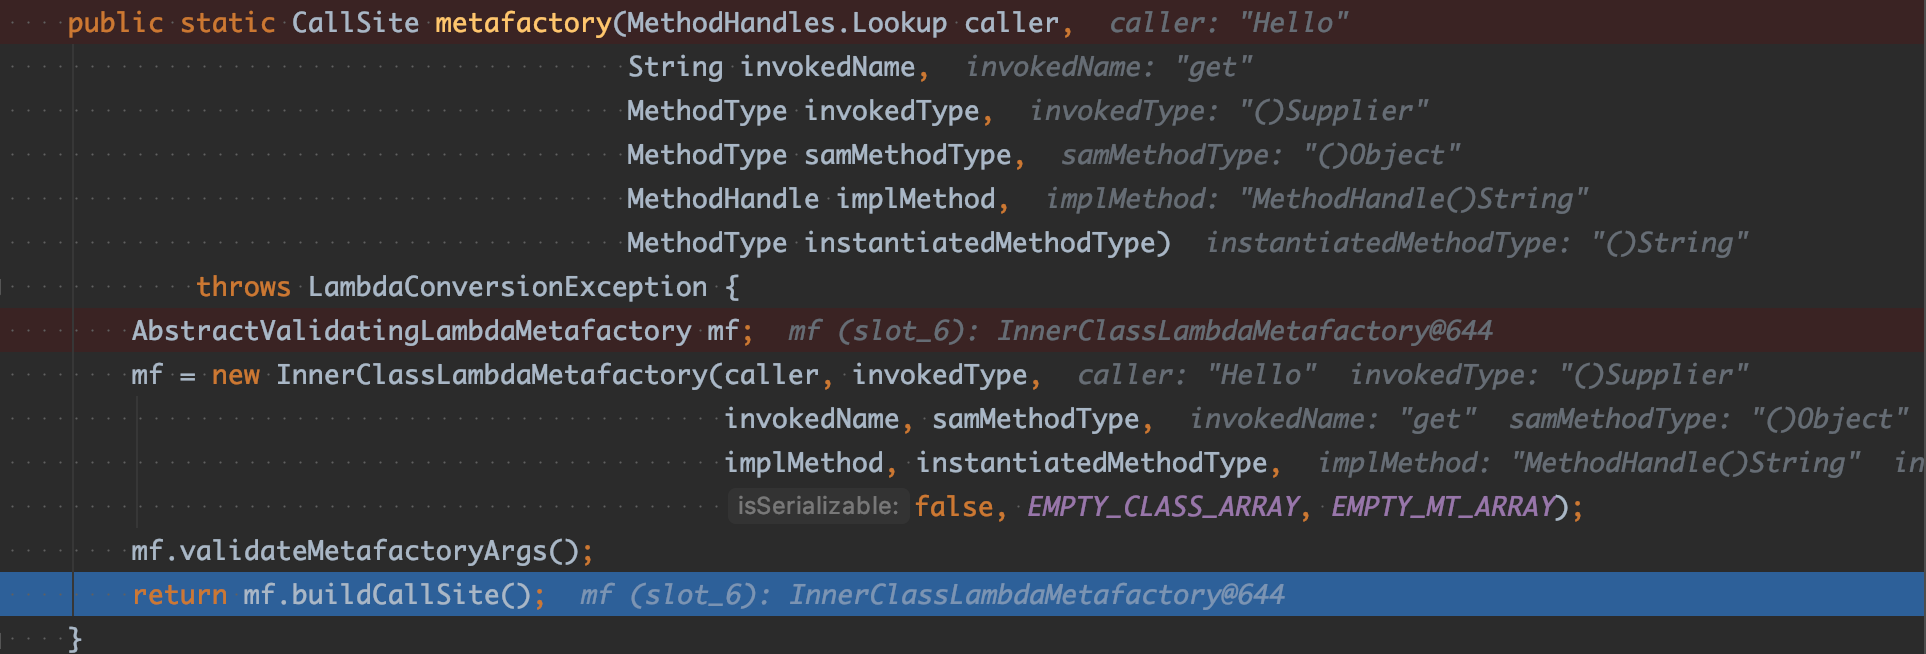
\includegraphics[keepaspectratio,alt={Debug metafactory}]{images/debug_metafactory.png}}
\caption{Debug metafactory}
\end{figure}

在这个类里面创建了一个匿名类，并通过\texttt{UNSAFE.ensureClassInitialized(innerClass)}直接加载到JVM中，没有出现在class文件中，不过通过jvm参数可以输出出来：

\begin{Shaded}
\begin{Highlighting}[]
\ExtensionTok{java} \AttributeTok{{-}Djdk.internal.lambda.dumpProxyClasses}\OperatorTok{=}\NormalTok{/Users/hfli/Downloads/tmp Hello}
\end{Highlighting}
\end{Shaded}

这样会生成一个\texttt{Hello\$\$Lambda\$1.class}的文件，反编译这个类可以看到如下的信息：

\begin{Shaded}
\begin{Highlighting}[]
\DataTypeTok{final} \KeywordTok{class}\NormalTok{ Hello$$Lambda$}\DecValTok{1} \KeywordTok{implements}\NormalTok{ Supplier }\OperatorTok{\{}
    \KeywordTok{private}\NormalTok{ Hello$$Lambda$}\DecValTok{1}\OperatorTok{()} \OperatorTok{\{}
    \OperatorTok{\}}

    \AttributeTok{@Hidden}
    \KeywordTok{public} \BuiltInTok{Object} \FunctionTok{get}\OperatorTok{()} \OperatorTok{\{}
        \ControlFlowTok{return}\NormalTok{ Hello}\OperatorTok{.}\FunctionTok{lambda}\NormalTok{$main$}\DecValTok{0}\OperatorTok{();}
    \OperatorTok{\}}
\OperatorTok{\}}
\end{Highlighting}
\end{Shaded}

这里实际是包装了一下\texttt{Supplier}接口，而具体调用的\texttt{Hello.lambda\$main\$0()}方法，可以在\texttt{Hello.class}文件中看到（需要使用\texttt{javap\ -p}选项输出私有方法):

\begin{verbatim}
private static java.lang.String lambda$main$0();
    descriptor: ()Ljava/lang/String;
    flags: ACC_PRIVATE, ACC_STATIC, ACC_SYNTHETIC
    Code:
      stack=1, locals=0, args_size=0
         0: ldc           #7                  // String Hello world!
         2: areturn
      LineNumberTable:
        line 6: 0
\end{verbatim}

所以大致是这个样子的过程：

\begin{itemize}
\tightlist
\item
  调用lambda时，首先通过找到对应的引导方法（也就是\texttt{metafactory()})，开始执行
\item
  JVM生成一个匿名类\texttt{Hello\$\$Lambda\$1}，这个类中包含了lambda的实际实现
\item
  创建一个CallSite，绑定到一个MethodHandle指向这个匿名类的实现\texttt{Hello\$\$Lambda\$1.get()}。这里引导方法就调用完成了
\item
  这个MethodHandle指向的方法被执行，调用到\texttt{Hello.lambda\$main\$0()}关联的字节码，得到最终的结果
\end{itemize}

值得注意的是，引导方法只需要执行一次，如果一个lambda执行了多次，那么只有第一次会去调用引导方法生成CallSite，以后都可以直接拿来使用了。

\section{结语}\label{ux7ed3ux8bed}

通过上面的描述，相信大家对\texttt{invokedynamic}有了一个粗略的了解，但要真正深入去了解的话，还是有很多东西需要去了解和研究的。虽然\texttt{invokedynamic}指令很强大，给了JVM的开发者很大的自由度，但实际上对于Java程序员来说，并没有太多可以操控的东西。如同上面提到的Duck Typing，在C\#中可以这样：

\begin{Shaded}
\begin{Highlighting}[]
\NormalTok{Object obj }\OperatorTok{=} \OperatorTok{...;} \CommentTok{// no static type available }
\NormalTok{dynamic duck }\OperatorTok{=}\NormalTok{ obj}\OperatorTok{;}
\NormalTok{duck}\OperatorTok{.}\FunctionTok{quack}\OperatorTok{();}     \CommentTok{// or any method. no compiler checking.}
\end{Highlighting}
\end{Shaded}

可能我们永远也没法使用Java来完成同样的任务，也许有一部分人会比较失望，但本身这是一把双刃剑，我还是倾向\href{http://www.yinwang.org/blog-cn/2016/01/18/java}{给Java说句公道话}。而借助于JVM平台，我们实际上有了越来越多的选择，Scala, Kotlin，Groovy等等。可以说从某个方面来讲，正是Java决策者对于每一个决策的慎重，才造就了今天Java程序员不愁饭吃的局面。

\begin{quote}
``When you have 9 million programmers using your language and out of which 1 million programmers know where you live you have to decide things differently.'' ------\href{https://www.youtube.com/watch?v=1OpAgZvYXLQ&t=1993s}{Venkat Subramaniam}
\end{quote}

参考文章：

\begin{itemize}
\tightlist
\item
  \href{https://www.infoq.com/articles/Invokedynamic-Javas-secret-weapon/}{Invokedynamic - Java's Secret Weapon}
\item
  \href{https://stackoverflow.com/questions/6638735/whats-invokedynamic-and-how-do-i-use-it}{What's invokedynamic and how do I use it?}
\item
  \href{https://zh.wikipedia.org/wiki/\%E9\%B8\%AD\%E5\%AD\%90\%E7\%B1\%BB\%E5\%9E\%8B}{Duck Typing - Wiki}
\item
  \href{https://devopedia.org/duck-typing}{Duck Typing}
\item
  \href{http://blog.headius.com/2008/09/first-taste-of-invokedynamic.html}{A First Taste of InvokeDynamic}
\item
  \href{https://www.javacodegeeks.com/2012/02/java-7-complete-invokedynamic-example.html}{Java 7: A complete invokedynamic example}
\item
  \href{https://my.oschina.net/lt0314/blog/3146028}{你不知道Lambda的秘密和陷阱}
\item
  \href{http://wiki.jvmlangsummit.com/images/9/93/2011_Forax.pdf}{JSR 292 Cookbook}
\item
  \href{https://www.jianshu.com/p/d74e92f93752}{理解 invokedynamic}
\end{itemize}

邮件阅读体验不佳，如需更好体验可以移步 \href{https://riguz.com/it/java/java_invokedynamic/}{在线版本}


\end{document}
